%PREAMBLE
\begin{comment}
%\documentclass[11pt]{article}
%\newcommand{\pablo}[1]{\textcolor{blue}{{\bf  #1}}}
\newcommand{\carlos}[1]{\textcolor{red}{{\bf  #1}}}
\newcommand{\fabio}[1]{\textcolor{purple}{{\bf  #1}}}
\newcommand{\susana}[1]{\textcolor{violet}{{\bf  #1}}}

% HEP names :: https://ctan.javinator9889.com/macros/latex/contrib/hepnames/hepnames.pdf

\DeclarePairedDelimiter\bra{\langle}{\rvert}
\DeclarePairedDelimiter\ket{\lvert}{\rangle}
\DeclarePairedDelimiterX\braket[2]{\langle}{\rangle}{#1 \delimsize\vert #2}

\newcommand*{\yt}{\ensuremath{y_{t}}\xspace}
\newcommand*{\tchannel}{\ensuremath{t\text{-channel}}\xspace}
\newcommand*{\schannel}{\ensuremath{s\text{-channel}}\xspace}
%\newcommand*{\lepT}{\ensuremath{\Pl_{\Pt}}\xspace}
%\newcommand*{\lepH}{\ensuremath{\Pl_{\PHiggs}}\xspace}

%\newcommand*{\muR}{\ensuremath{\mu_{\text{R}}}\xspace}
%\newcommand*{\muF}{\ensuremath{\mu_{\text{F}}}\xspace}

% Add external packages
\usepackage[italic]{hepnicenames}

%%%%%%%%%%%%%%%%%%%%%%%
%  From NA-HIGG-2020-02-INT1-defs.sty    %
%%%%%%%%%%%%%%%%%%%%%%%
% Basic tHq-related macros
%\newcommand*{\tHq}{\ensuremath{\Pqt{}\PH{}\Pq}\xspace}
%\newcommand*{\tHq}{\ensuremath{\Ptop \PHiggs \Pq}\xspace}
%\newcommand*{\tHq}{\Pqt{}\PH{}\Pq}
\newcommand*{\tHq}{\ensuremath{tHq}\xspace}
\newcommand*{\tH}{\ensuremath{\Pqt{}\PH{}}\xspace}
\newcommand*{\tHqsec}{\texorpdfstring{\Pqt{}\PH{}\Pq}{tHq}}
\newcommand*{\tHqML}{\ensuremath{\Pqt{}\PH{}\Pq\,(\text{ML})}\xspace}
\newcommand*{\tHqbb}{\ensuremath{\Pqt{}\PH{}\Pq\,(\bbbar)}\xspace}
\newcommand*{\tbarHq}{\Paqt{}\PH{}Pq}
\newcommand*{\tHbb}{\ensuremath{\tHq (\PH \to \bbbar)}\xspace}
\newcommand*{\tHtautau}{\ensuremath{\tHq (\PH \to \Pgt{}\Pgt)}\xspace}
\newcommand*{\dR}{\ensuremath{\Delta R}\xspace}
\newcommand*{\trexfitter}{TRExFitter\xspace}
\newcommand*{\thqloop}{\texttt{tHqLoop}\xspace}


\newcommand*{\MpT}{\ensuremath{\vec{p}_{\text{T}}^{\text{miss}}}\xspace}
\newcommand*{\mtw}{\ensuremath{m_{\text{T}}(\Pl,\MET)}}
\newcommand*{\mlb}{\ensuremath{m_{\Pl\Pqb}}}
\newcommand*{\mOSSF}{\ensuremath{m_{\text{OSSF}}}\xspace}

% Background processes
\newcommand*{\ttX}{\ensuremath{\Pqt{}\Paqt{}X}\xspace}
\newcommand*{\tX}{\ensuremath{\Pqt{}X}\xspace}

%\newcommand*{\ttX}{\Pqt{}\Paqt{}+X}
\newcommand*{\ttH}{\Pqt{}\Paqt{}\PH}
%\newcommand*{\ttH}{\ensuremath{\Pqt{}\Paqt{}\PH}\xspace}
\newcommand*{\ttZ}{\Pqt{}\Paqt{}\PZ}
\newcommand*{\ttV}{\ensuremath{\Pqt{}\Paqt{}V}\xspace}
\newcommand*{\ttW}{\Pqt{}\Paqt{}\PW}
\newcommand*{\ttWj}{\ensuremath{t\bar{t}W+j}\xspace}
\newcommand*{\tZq}{\Pqt{}\PZ{}\Pq}
\newcommand*{\tWZ}{\Pqt{}\PW{}\PZ}
\newcommand*{\tWH}{\Pqt{}\PW{}\PH}
\newcommand*{\tHW}{\Pqt{}\PW{}\PH}
\newcommand*{\tW}{\Pqt{}\PW}
\newcommand*{\Wt}{\Pqt{}\PW}
\newcommand*{\diboson}{diboson\xspace}
\newcommand*{\Diboson}{Diboson\xspace}
\newcommand*{\triboson}{triboson\xspace}
\newcommand*{\Triboson}{Triboson\xspace}
\newcommand*{\Vjets}{\ensuremath{V\text{+\,jets}}\xspace}

\newcommand*{\ttt}{\ensuremath{ttt}\xspace}
\newcommand*{\tttt}{\ensuremath{t\bar{t}t\bar{t}}\xspace}
\newcommand*{\ggH}{\ensuremath{ggH}\xspace}
\newcommand*{\qqH}{\ensuremath{qqH}\xspace}
\newcommand*{\WH}{\ensuremath{WH}\xspace}
\newcommand*{\ZH}{\ensuremath{ZH}\xspace}

% Fake leptons
\newcommand*{\elHF}{\ensuremath{e_{\text{HF}}}\xspace}
\newcommand*{\muHF}{\ensuremath{\mu_{\text{HF}}}\xspace}
\newcommand*{\elCo}{\ensuremath{e_{\text{conv}}}\xspace} 
\newcommand*{\kelHF}{\ensuremath{\mu(e_{\text{HF}})}\xspace}
\newcommand*{\kmuHF}{\ensuremath{\mu(\mu_{\text{HF}})}\xspace}
\newcommand*{\kelCo}{\ensuremath{\mu(e_{\text{conv}})}\xspace} 

% Signal regions
\newcommand*{\dileptau}{\ensuremath{2\Pl+1\tauhad}\xspace}
\newcommand*{\dilepOStau}{\ensuremath{2\Pl\,\text{OS}+1\tauhad}\xspace}
\newcommand*{\dilepSStau}{\ensuremath{2\Pl\,\text{SS}+1\tauhad}\xspace}

\newcommand*{\onelep}{\ensuremath{1\Pl}\xspace}
\newcommand*{\dilep}{\ensuremath{2\Pl}\xspace}
\newcommand*{\dilepOS}{\ensuremath{2\Pl\,\text{OS}}\xspace}
\newcommand*{\dilepSS}{\ensuremath{2\Pl\,\text{SS}}\xspace}
%\newcommand*{\SS}{\ensuremath{\text{SS}}\xspace}
%\newcommand*{\OS}{\ensuremath{\text{OS}}\xspace}

\newcommand*{\trilep}{\ensuremath{3\Pl}\xspace}
\newcommand*{\lepditau}{\ensuremath{1\Pl+2\tauhad}\xspace}




\newcommand*{\lumi}{\ensuremath{\mathcal{L}}\xspace}
\newcommand*{\lumiunits}{$\,$ cm$^{2} \,$s$^{-1}$\xspace}


%Other
\newcommand*{\CM}{\ensuremath{\sqrt{s}}\xspace}
 
\newcommand*{\Wtb}{\ensuremath{tWb}\xspace}
\newcommand*{\tWb}{\Wtb}
%\newcommand*{\tWb}{\ensuremath{tWb}\xspace}
\newcommand*{\pfour}{\ensuremath{\boldsymbol{\textrm{p}}}\xspace} 

\newcommand*{\tchan}{\ensuremath{t}-channel}
\newcommand*{\mtop}{\ensuremath{m_{\Ptop}}\xspace}
%\newcommand*{\mH}{\ensuremath{m_H}\xspace}
%\newcommand*{\HT}{\ensuremath{H_{\text{T}}}\xspace}

%\newcommand*{\PWplus}{\ensuremath{\PW^{+}}\xspace}
%\newcommand*{\PWminus}{\ensuremath{\PW^{-}}\xspace}
%\newcommand*{\Pgamma}{\ensuremath{\gamma}\xspace}

 \newcommand*{\greekphys}{\ensuremath{\varphi\upsilon\sigma\iota\kappa \eta}\xspace}
 \newcommand*{\greekatom}{\ensuremath{\alpha \tau o \mu o \nu}\xspace}
 \newcommand{\emu}{\ensuremath{\Pe/\Pmu}\xspace}

\newcommand*{\momentum}{\ensuremath{\overrightarrow{p}}\xspace} 
%\newcommand*{\CP}{\ensuremath{\mathcal{CP}}\xspace}
\newcommand*{\CP}{CP\xspace}

% Decays (Please, check latex/atlasprocess.sty and latex/atlasparticle.sty for more definitions!)
\newcommand{\bb}{\ensuremath{\Pqb\Paqp}\xspace}
\newcommand{\WW}{\ensuremath{\PW\PW^{*}}\xspace}
\newcommand{\ZZ}{\ensuremath{\PZ\PZ^{*}}\xspace}
\newcommand{\Higgsdecays}{\ensuremath{\PH \rightarrow b\bar{b}, \WW, \ZZ, \tau\tau}\xspace}
\newcommand{\Higgsdecayslep}{\ensuremath{\PH \rightarrow \WW, \ZZ, \tau\tau}\xspace}
\newcommand{\HWW}{\ensuremath{\PH \rightarrow \WW}\xspace}
\newcommand{\HZZ}{\ensuremath{\PH \rightarrow \ZZ}\xspace}

% reconstruction definitions
\newcommand{\pnutop}{\ensuremath{\vec{p^{\Pnu, \text{top}}}}\xspace}
\newcommand{\pnutopx}{\ensuremath{p^{\Pnu, \text{top}}_x}\xspace}
\newcommand{\pnutopy}{\ensuremath{p^{\Pnu, \text{top}}_y}\xspace}
\newcommand{\pnutopz}{\ensuremath{p_{z}(\Pnu_{\text{top}})}\xspace}
\newcommand{\pnutopT}{\ensuremath{\pT(\Pnu_{\text{top}})}\xspace}
\newcommand{\phinutop}{\ensuremath{\phi(\Pnu_{\text{top}})}\xspace}
\newcommand{\pltop}{\ensuremath{\vec{p^{\Plepton, \text{top}}}}\xspace}
\newcommand{\pltopx}{\ensuremath{p^{\Plepton, \text{top}}_x}\xspace}
\newcommand{\pltopy}{\ensuremath{p^{\Plepton, \text{top}}_y}\xspace}
\newcommand{\pltopz}{\ensuremath{p^{\Plepton, \text{top}}_z}\xspace}
\newcommand{\pltopT}{\ensuremath{\pT(\Plepton_{\text{top}})}\xspace}
\newcommand{\philtop}{\ensuremath{\phi(\ell_{\text{top}})}\xspace}
\newcommand{\phibtop}{\ensuremath{\phi(b_{\text{top}})}\xspace}
\newcommand{\tauvis}{\ensuremath{\Ptau_{\text{vis}}}\xspace}

\newcommand{\leptop}{\ensuremath{\Plepton^{\text{top}}}\xspace}
\newcommand{\lepH}{\ensuremath{{\Plepton^{\PH}}}\xspace}
\newcommand{\Hvismass}{\ensuremath{m_{\PH}^{\text{vis}}}\xspace}
\newcommand{\toprecomass}{\ensuremath{\mtop^{\text{reco}}}\xspace}
% \newcommand{\toprecomass}{\ensuremath{\Pqt_{\text{reco}}^{\text{m}}\xspace}}
% \newcommand{\Hvismass}{\ensuremath{\PH_{\text{vis}}^{\text{m}}\xspace}}
\newcommand{\MMC}{\texttt{MissingMassCalculator}\xspace}

% luminosity (2015)
\newcommand{\lumiFifteenRelUnc}{1.13} % in [%]
\newcommand{\lumitagFifteen}{{\small\texttt{OfLumi-13TeV-008}}}
%\newcommand{\lumiFifteenInPbNoUnits}{3219.56}
%\newcommand{\lumiFifteenInFbNoUnits}{3.2}
\newcommand{\lumiFifteenInPbNoUnits}{3244.54} % final luminosity recommendation for Run 2 analyses (https://twiki.cern.ch/twiki/bin/viewauth/Atlas/LuminosityForPhysics#2015_2018_13_TeV_proton_proton_f)
\newcommand{\lumiFifteenInFbNoUnits}{3.2}
%\newcommand{\dataperiodsFifteen}{D--J}
\newcommand{\dataperiodsFifteen}{D--H,J}
\newcommand{\firstdatarunFifteen}{276262}
\newcommand{\lastdatarunFifteen}{284484}
\newcommand{\datarunsFifteen}{\firstdatarunFifteen--\lastdatarunFifteen}
\newcommand{\dataeventsFifteen}{220.58M}

% luminosity (2016)
\newcommand{\lumiSixteenRelUnc}{0.89} % in [%]
\newcommand{\lumitagSixteen}{{\small\texttt{OfLumi-13TeV-009}}}
%\newcommand{\lumiSixteenInPbNoUnits}{32988.1}
%\newcommand{\lumiSixteenInFbNoUnits}{33.0}
% final luminosity recommendation for Run 2 analyses (https://twiki.cern.ch/twiki/bin/viewauth/Atlas/LuminosityForPhysics#2015_2018_13_TeV_proton_proton_f)
\newcommand{\lumiSixteenInPbNoUnits}{33402.2}
\newcommand{\lumiSixteenInFbNoUnits}{33.4}
%\newcommand{\dataperiodsSixteen}{A--L}
\newcommand{\dataperiodsSixteen}{A--G,I,K,L}
\newcommand{\firstdatarunSixteen}{297730}
\newcommand{\lastdatarunSixteen}{311481}
\newcommand{\datarunsSixteen}{\firstdatarunSixteen--\lastdatarunSixteen}
\newcommand{\dataeventsSixteen}{1057.84M}

% luminosity (2017)
\newcommand{\lumiSeventeenRelUnc}{1.13} % in [%]
\newcommand{\lumitagSeventeen}{{\small\texttt{OfLumi-13TeV-010}}}
%\newcommand{\lumiSeventeenInPbNoUnits}{44307.4}
%\newcommand{\lumiSeventeenInFbNoUnits}{44.3}
% final luminosity recommendation for Run 2 analyses (https://twiki.cern.ch/twiki/bin/viewauth/Atlas/LuminosityForPhysics#2015_2018_13_TeV_proton_proton_f)
\newcommand{\lumiSeventeenInPbNoUnits}{44630.6}
\newcommand{\lumiSeventeenInFbNoUnits}{44.6} 
%\newcommand{\dataperiodsSeventeen}{B--K}
\newcommand{\dataperiodsSeventeen}{B--F,H,I,K}
\newcommand{\firstdatarunSeventeen}{325713}
\newcommand{\lastdatarunSeventeen}{340453}
\newcommand{\datarunsSeventeen}{\firstdatarunSeventeen--\lastdatarunSeventeen}
%%%\newcommand{\datarunsSeventeen}{324320--341649}
\newcommand{\dataeventsSeventeen}{1340.80M}

% luminosity (2018)
\newcommand{\lumiEightteenRelUnc}{1.10} % in [%]
\newcommand{\lumitagEightteen}{{\small\texttt{OfLumi-13TeV-010}}}
%\newcommand{\lumiEightteenInPbNoUnits}{58450.1}
%\newcommand{\lumiEightteenInFbNoUnits}{58.5}
% final luminosity recommendation for Run 2 analyses (https://twiki.cern.ch/twiki/bin/viewauth/Atlas/LuminosityForPhysics#2015_2018_13_TeV_proton_proton_f)
\newcommand{\lumiEightteenInPbNoUnits}{58791.6}
\newcommand{\lumiEightteenInFbNoUnits}{58.8}
\newcommand{\lumiEightteenInPb}{\SI{\lumiEightteenInPbNoUnits}{\per\pb}}
\newcommand{\lumiEightteenInFb}{\SI{\lumiEightteenInFbNoUnits}{\per\fb}}
%\newcommand{\dataperiodsEightteen}{B--Q}
\newcommand{\dataperiodsEightteen}{B--D,F,I,K,L,M,O,Q}
\newcommand{\firstdataruEightteen}{348885}
\newcommand{\lastdatarunEightteen}{364292}
\newcommand{\datarunsEightteen}{\firstdataruEightteen--\lastdatarunEightteen}
%%%\newcommand{\datarunsEightteen}{348197--364292}
\newcommand{\dataeventsEightteen}{1716.77M}

% luminosity (2015+2016+2017)
%\newcommand{\lumiInPb}{80515.06~\invpb}
% \newcommand{\partlumi}{\SI{80.52}{\per\fb}}
%\newcommand{\datafirstyear}{2015}
%\newcommand{\datalastyear}{2017}

% luminosity (2015+2016+2017+2018)
%
% https://twiki.cern.ch/twiki/bin/viewauth/Atlas/LuminosityForPhysics#2015_2018_13_TeV_proton_proton_f
% final luminosity recommendation for Run 2 analyses (central value + uncertainty)
\newcommand{\lumiRelUnc}{0.83} % in [%]
\newcommand{\lumiInPbNoUnits}{140068.94} % in pb-1
\newcommand{\lumiInFbNoUnits}{140} % in fb-1
\newcommand{\lumiWithUnc}{\ensuremath{140.1 \pm 1.2}\,\si{\per\fb}} % in fb-1
%
% old recommendation
%\newcommand{\lumiRelUnc}{1.7} % in [%]
%\newcommand{\lumiInPbNoUnits}{138965.16} % in pb-1
%\newcommand{\lumiInFbNoUnits}{139} % in fb-1
%\newcommand{\lumiWithUnc}{\ensuremath{\lumiInFbNoUnits \pm 2.4}\,\si{\per\fb}} % in fb-1
\newcommand{\dataeventsAll}{4335.99M}
%
\newcommand{\lumiInPb}{\SI{\lumiInPbNoUnits}{\per\pb}}
%\newcommand{\lumi}{\SI{\lumiInFbNoUnits}{\per\fb}}
\newcommand{\datafirstyear}{2015}
\newcommand{\datalastyear}{2018}

% % tunes and PDF sets
\def\cteq{CTEQ6L1\xspace}
\def\ctten{CT10\xspace}
\def\cttennlo{CT10\,NLO\xspace}
\def\cttennnlo{CT10\,NNLO\xspace}
\def\ctfourteennlo{CT14\,NLO\xspace}
\def\ctfourteennnlo{CT14\,NNLO\xspace}
\def\nnpdfnnlo{NNPDF3.0\,NNLO\xspace}
\def\nnpdfnlofourflav{NNPDF3.0\,NLO\,nf4\xspace}
\def\nnpdfnlo{NNPDF3.0\,NLO\xspace}
\def\nnpdftwonlo{NNPDF2.3\,NLO\xspace}
\def\nnpdftwo{NNPDF2.3\,LO\xspace}
\def\nnpdftwofiveflav{NNPDF2.3\,5f\,FFN\xspace}
\def\mstw{MSTW2008\,NLO\xspace}
\def\a14{A14\xspace}
\def\auet{AUET2\xspace}
\def\aznlo{AZNLO\xspace}
\def\mmhtnnlo{MMHT2014\,NNLO\xspace}
\def\mmhtnlo{MMHT2014\,NLO\xspace}
\def\mmhtlo{MMHT2014\,LO\xspace}
\def\mstwnlo{MSTW2008\,68\%\,CL\,NLO \xspace}
\def\mstwnnloninety{MSTW2008\,90\%\,CL\,NNLO \xspace}
\def\ueee{UE-EE-5\xspace}




 
\endinput


%\begin{document}
asdf
%ENDPREAMBLE
\end{comment}

\chapter{Effect of negative weights}
%\tableofcontents
\label{chap:Appendix:NegWeights}

%\pablo{Igual esto se puede integrar en la sección~\ref{sec:Chap3.1:Data:Model}. }


%%%%%%%%%%%%%%%%%%%%%
%         Neg Weights  - Intro         %
%%%%%%%%%%%%%%%%%%%%%
\section{Negatively weighted events}
\label{chap:Appendix:NegWeights:intro}
%\begin{itemize}
%	\item What is a weight in a MC event?
%	\item Why are there negatively weighted events?
%	\item Why are negative weights problematic?
%\end{itemize}

The weight in a MC-simulated sample refers to a factor assigned to each 
event in the simulation to account for various effects such as event generation, 
detector response, and data-to-simulation discrepancies. These weights are used 
to scale the simulated events to better match the observed data or to accurately 
model specific physical processes or background contributions.  These negative weights reflect the cancellation 
of positive and negative contributions to ensure the correct overall probability distribution. 
The weights are derived based on theoretical calculations, detector simulations, and calibration 
procedures, and they are crucial for obtaining accurate predictions and comparisons 
with experimental data in analyses at ATLAS.
While negative weights pose challenges for statistical analysis and interpretation, they are necessary 
to accurately reproduce the expected physics processes and their interference effects. 

%It is important to handle negative weights properly in data analyses to avoid biases and ensure 
%reliable results. Various techniques and strategies are employed to mitigate the impact of negative
%weights, such as reweighting, rescaling, or event selection methods that minimise their impact on the final analysis.


% Good source: https://arxiv.org/pdf/2110.15211.pdf

The negative weighs can result in samples with reduced statistical power~\cite{Danziger:2021xvr}.
Therefore, the presence of negatively-weighted events, as opposed to exclusively positive-weight 
event samples, implies processing a significantly larger number of events to achieve comparable 
statistical significance. This issue is particularly pronounced during the final stage of detector simulation, 
where each event can require hours of CPU time~\cite{Andersen:2021mvw}.

Another problem with negative weights arises in the training of ML models, as it is further discussed
in Appendix~\ref{chap:Appendix:BDT}. 



%%%%%%%%%%%%%%%%%%%%%
%         Neg Weights  - Uncertainty         %
%%%%%%%%%%%%%%%%%%%%%
\section{Statistical uncertainty of negative weights}
\label{chap:Appendix:NegWeights:uncert}
Assume that there is a sample of $N$ MC-simulated events. Of these,
a fraction $x$ have negative weighs and, therefore, a fraction $(1-x)$ has a positive weight.
The effective number of events is $(N_{+} - N_{-})$, being $N_{+} = (1-x)N$ the amount of
positively weighted events and $N_{-} = xN$ the same for the negative weights.

The statistical fluctuations are calculated in terms of $x$ and the standard deviation 
($\sigma_{N}=\sqrt{N}$). The number of positive and negative events can fluctuate
randomly between $\pm \sigma_{-}$ for the later and  $\pm \sigma_{+}$ for the former.
Here, $\sigma_{-} = \sqrt{xN} = \sqrt{x}\,N$ and $\sigma_{+}= \sqrt{1-x}\,N$

The variance ($V=\sigma^{2}$) of the sample is then
\begin{equation*}%\label{eq:Appendix:NegWeights:varaince}
%\begin{split}
	V(N_{+} - N_{-}) = xV(N) + (1-x)V(N)= V(N)
%\end{split}
\end{equation*}
and the fractional uncertainty
\begin{equation*}%\label{eq:Appendix:NegWeights:StdDev}
%\begin{split}
	\frac{\sigma(N_{+} - N_{-})}{N_{+} - N_{-}} = \frac{\sigma_N}{(1-x)N - xN}
	= \frac{1}{1-2x}\frac{\sigma_n}{N}
%\end{split}
\end{equation*}
When the fraction of negative events is $x=0$, $\frac{\sigma(N_{+} - N_{-})}{N_{+} - N_{-}}
= \frac{\sigma_n}{N}$ as expected. In contrast, if $x=0.5$ the fractional uncertainty is infinite,
as expected.

For the signal \tHq \dileptau MC signal sample the fraction of negative weights is between 0.3 and 0.4 depending on the production used.
\begin{itemize}
	\item $x=0.3$	$\rightarrow$ $\frac{\sigma(N_{+} - N_{-})}{N_{+} - N_{-}}
	 = \frac{1}{0.2}\frac{\sigma_n}{N} = 5.0 \frac{\sigma_n}{N}$

	 \item $x=0.4$	$\rightarrow$ $\frac{\sigma(N_{+} - N_{-})}{N_{+} - N_{-}}
	 = \frac{1}{0.4}\frac{\sigma_n}{N} = 2.5 \frac{\sigma_n}{N}$
\end{itemize}

% All events VS positive weights only
The uncertainty of the effective number of events can be compared to that of using only the 
positively weighted events. If the two fractional uncertainties are divided:

\begin{equation*}
%\begin{split}
	\frac{\frac{\sigma(N_{+} - N_{-})}{N_{+} - N_{-}}}{\frac{\sigma(N_+)}{N_x}}=
	\frac{\frac{1}{1-2x}\frac{\sigma_n}{N}}{\frac{1}{\sqrt{(1-x)N}}} =
	\frac{\sqrt{1-x}}{1-2x} \frac{\sigma_n}{N} = \frac{\sqrt{1-x}}{1-2x}
%\end{split}
\end{equation*}
In the range of $x$ values for the \dileptau simulated signal events. 

\begin{minipage}[t]{0.57\linewidth}
\begin{itemize}
	\item $x=0.3$	$\rightarrow$ 
	$\frac{\frac{\sigma(N_{+} - N_{-})}{N_{+} - N_{-}}}{\frac{\sigma(N_+)}{N_x}}= 2.09$
	 \item $x=0.4$	$\rightarrow$ 
	$\frac{\frac{\sigma(N_{+} - N_{-})}{N_{+} - N_{-}}}{\frac{\sigma(N_+)}{N_x}}= 3.87$
\end{itemize}
\end{minipage}
\hfill
\raisebox{-1\baselineskip}{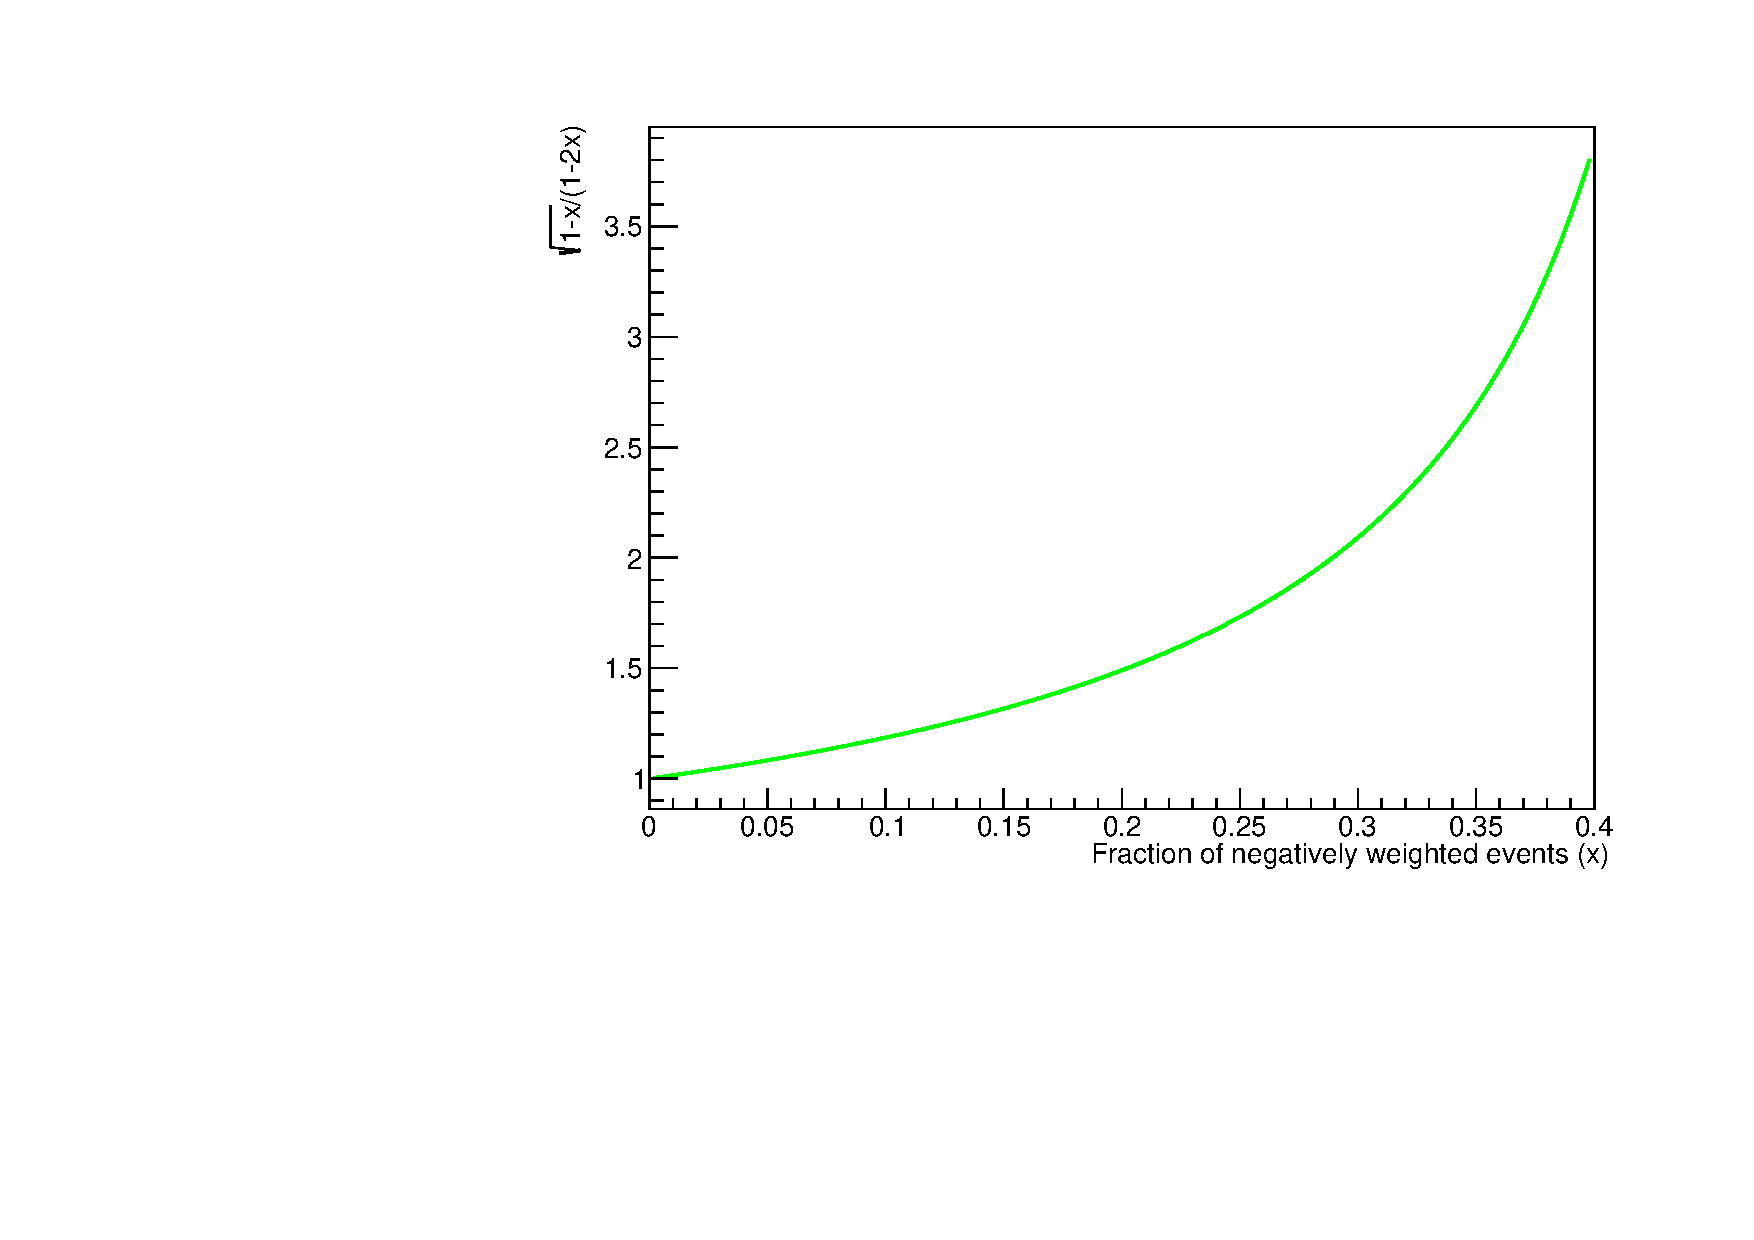
\includegraphics[width=0.35\textwidth]{Appendices/Appendix_NegativeWeigts/PosVsAll_err}}



In Figure~\ref{fig:Appendix:NegWeights:Distributions}, several $\Delta R$ distributions are generated using all the events
and just the positively weighted ones. As expected, the uncertainty bands are bigger for the 'All events' than for the
'Positive events'.  These histograms were produced to verify that using only the events with positive weights in
the training of the BDT for the lepton assignment in the SS scenario (Section~\ref{sec:ChaptH:Sig:LepAsign}) was not 
biasing the result. The size of the error bands is calculated by ROOT as the square root of the quadratic sum of the 
weights, as explained below.


\begin{figure}
\centering
\begin{subfigure}{.44\textwidth}
  \centering
  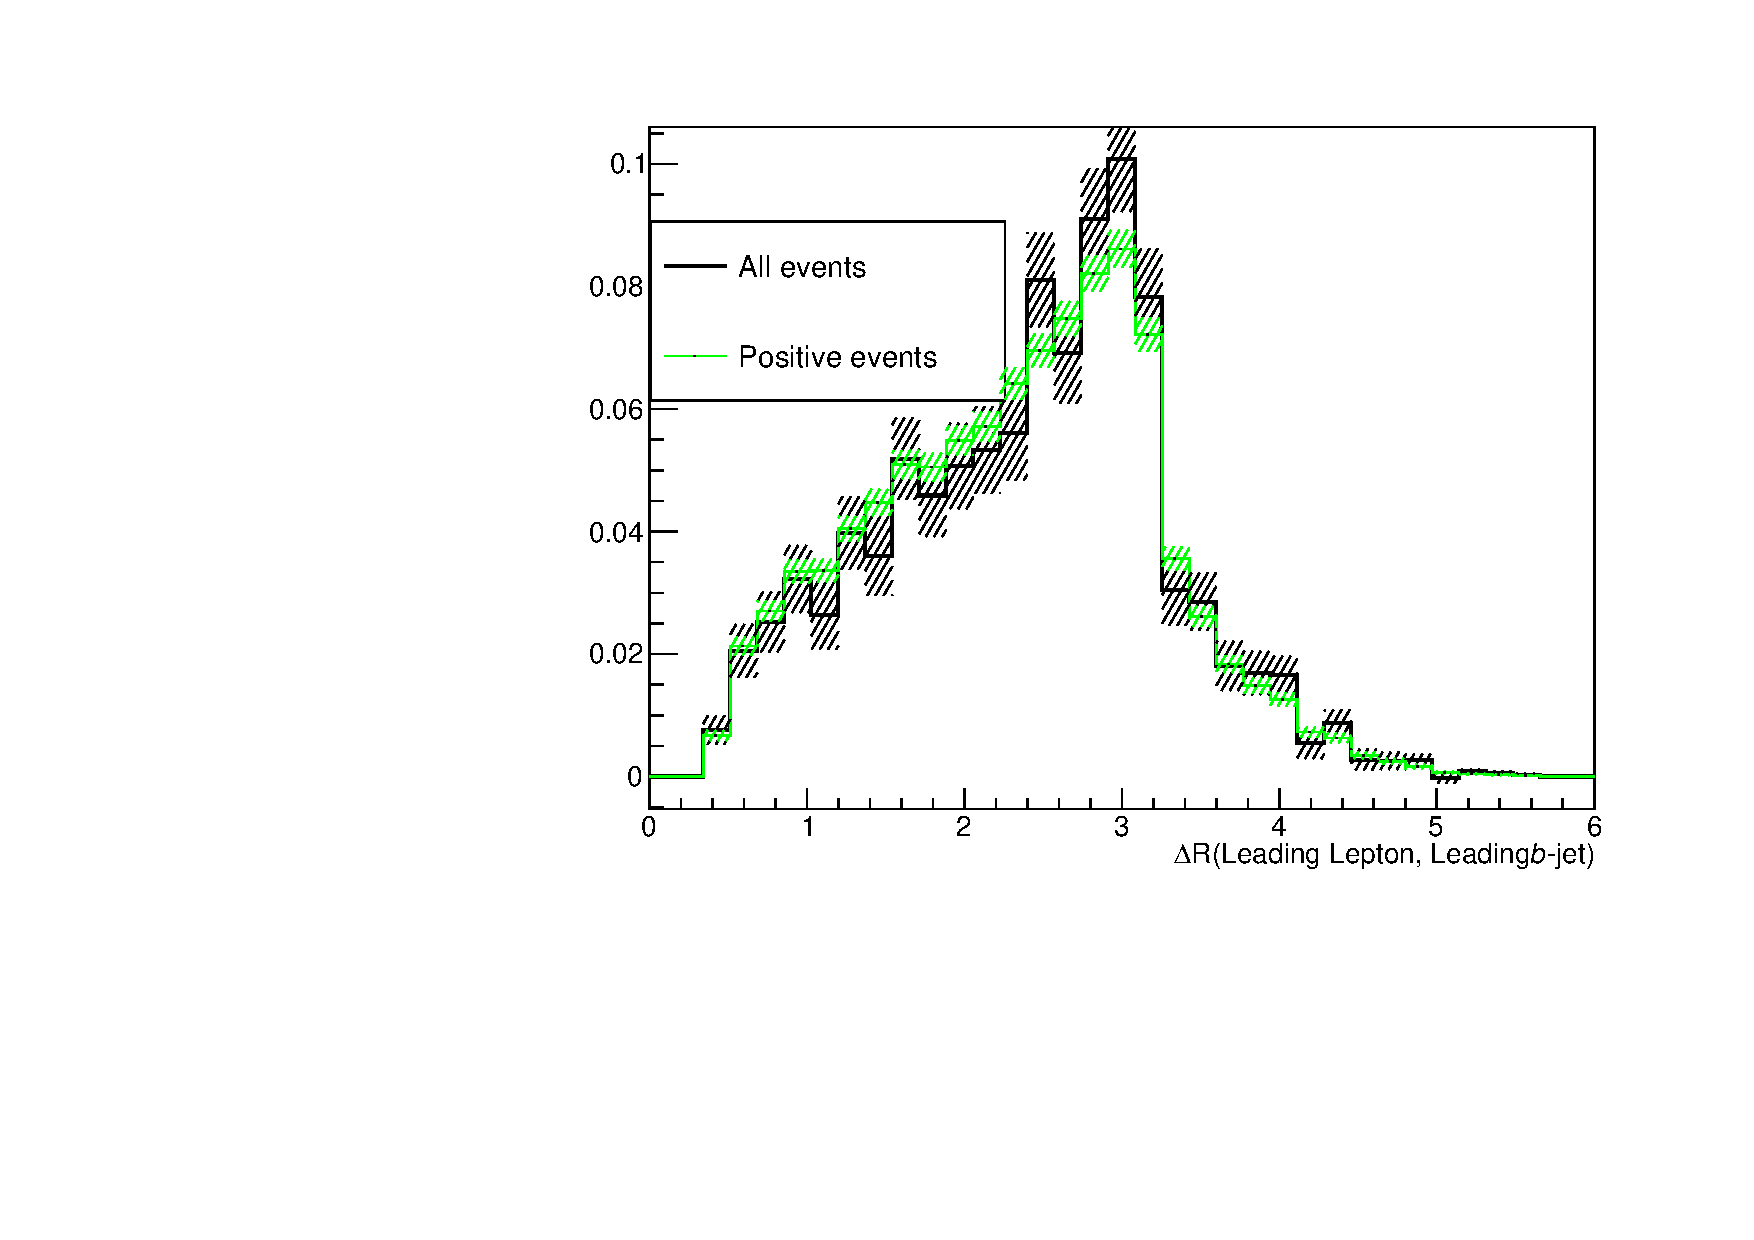
\includegraphics[width=.99\linewidth]{Appendices/Appendix_NegativeWeigts/PosVsAll_SS_err_deltaR_b_LightLep1}
  \caption{$\Delta R$(Leading light-favoured lepton, leading $b$-tagged jet)}
\end{subfigure}%
\begin{subfigure}{.44\textwidth}
  \centering
  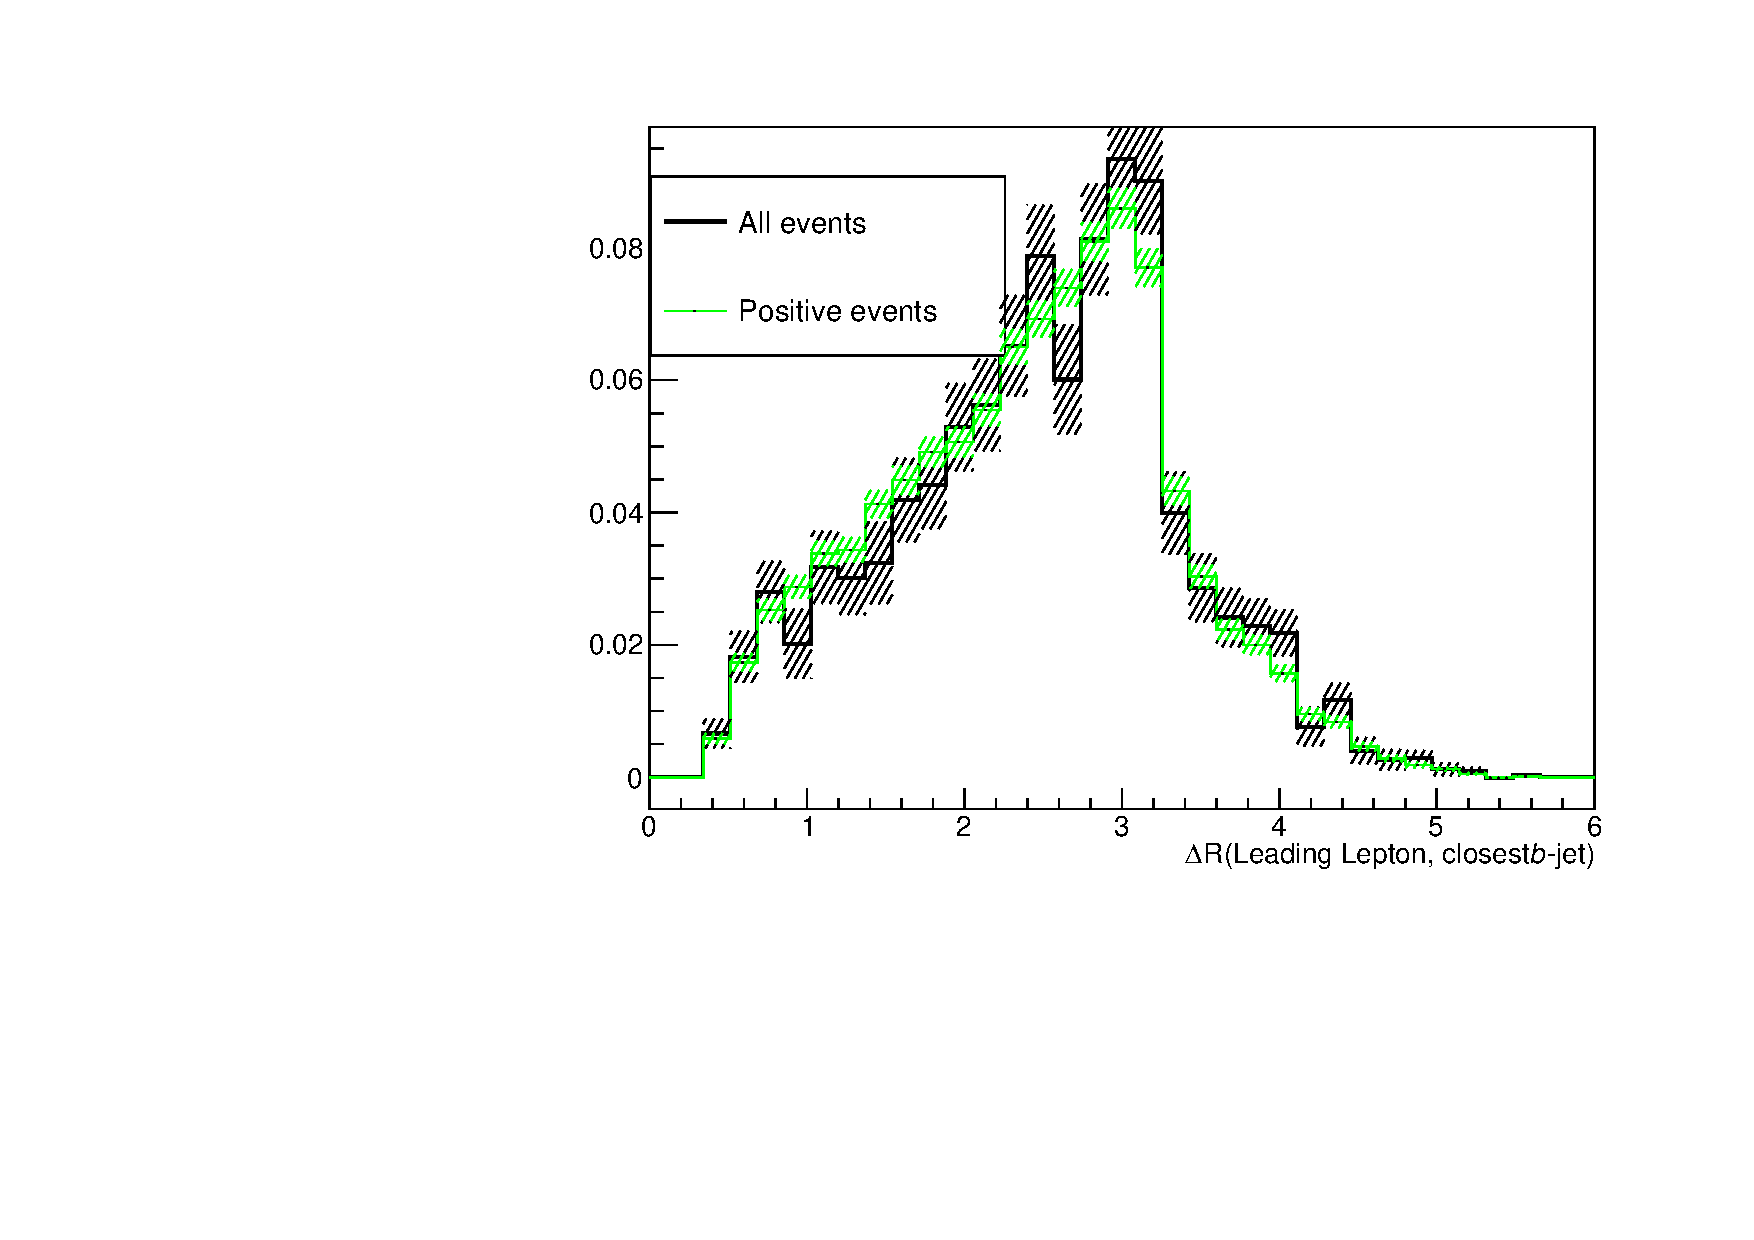
\includegraphics[width=.99\linewidth]{Appendices/Appendix_NegativeWeigts/PosVsAll_SS_err_DeltaRLeadingLeptonClosestBjet}
  \caption{$\Delta R$(Leading lepton, closest $b$-tagged jet)}
\end{subfigure} \hfill%

\begin{subfigure}{.44\textwidth}
  \centering
  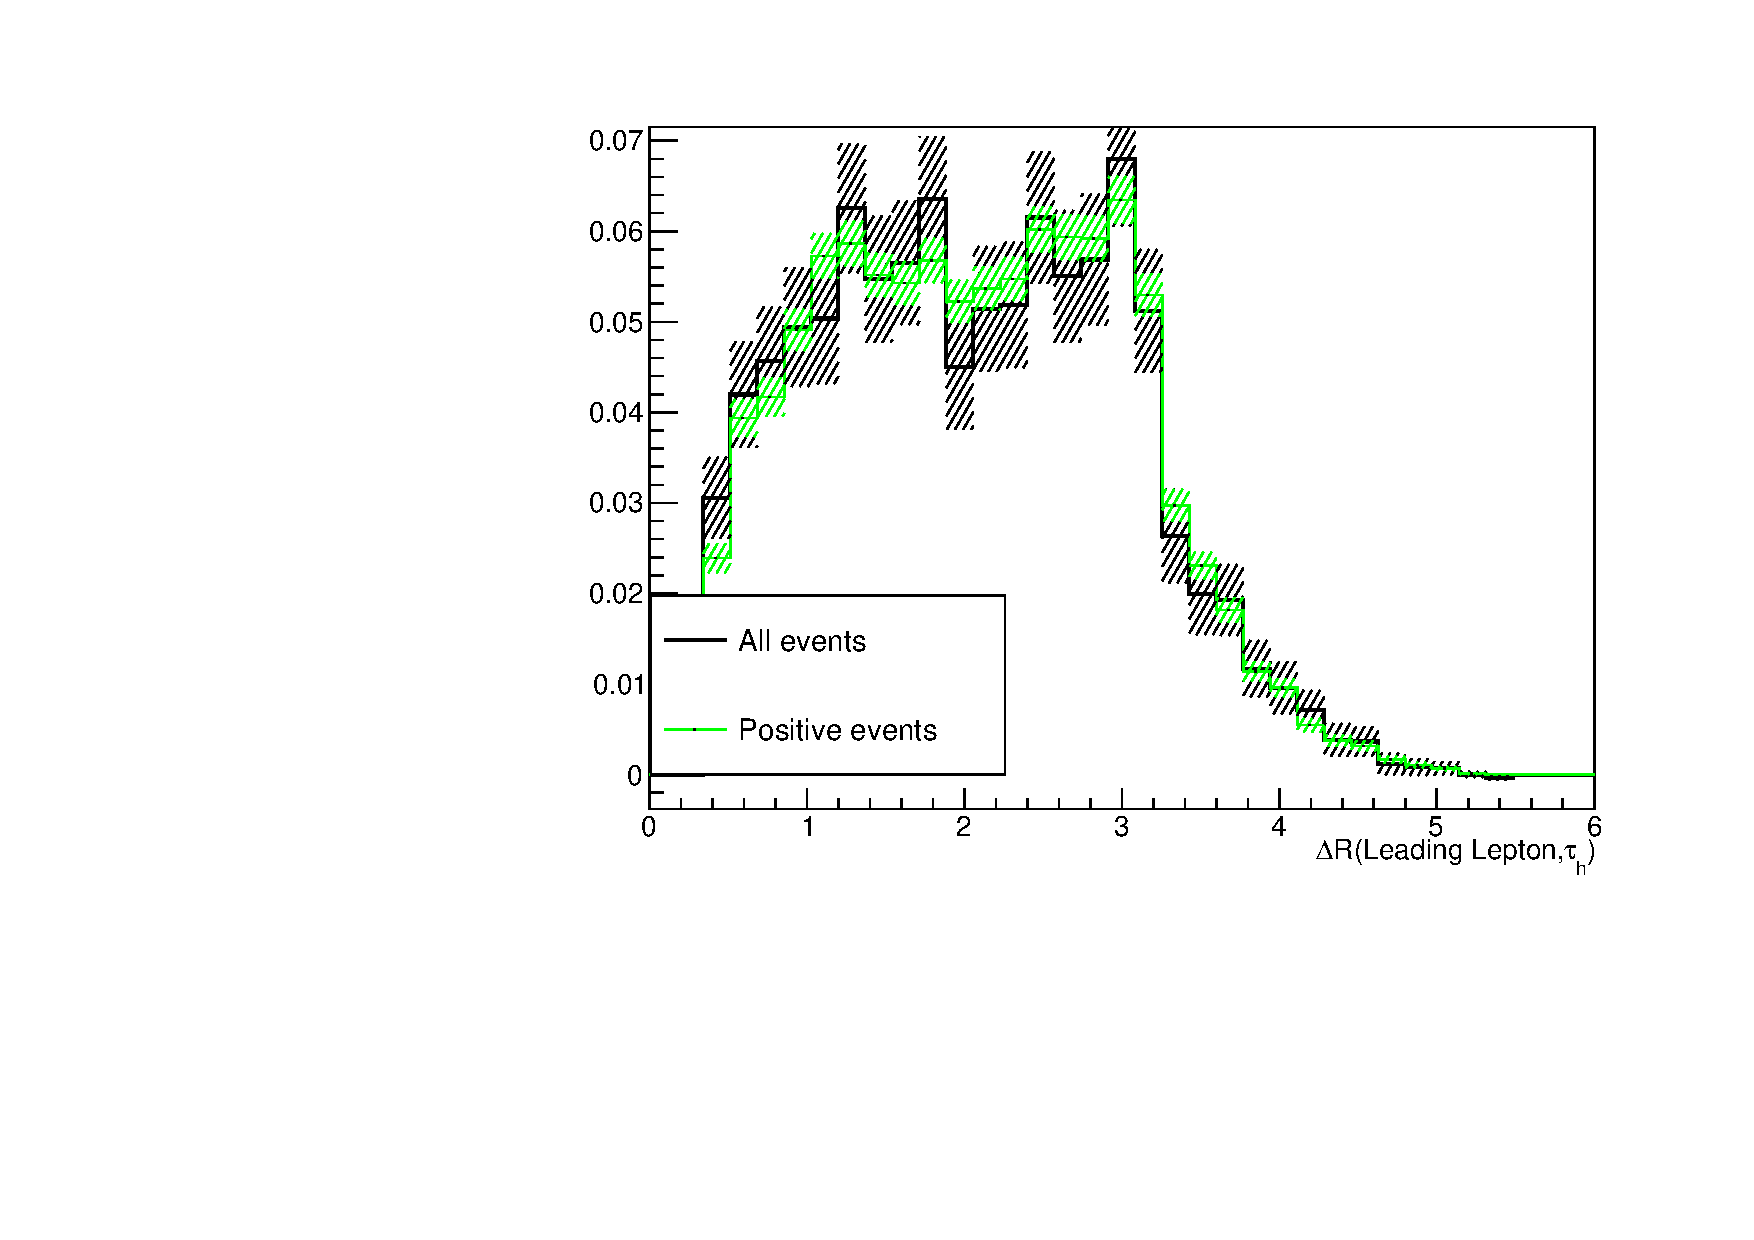
\includegraphics[width=.99\linewidth]{Appendices/Appendix_NegativeWeigts/PosVsAll_SS_err_deltaR_tau_LightLep1}
  \caption{$\Delta R$(\tauhad, Leading light-favoured lepton)}
\end{subfigure}%
\begin{subfigure}{.44\textwidth}
  \centering
  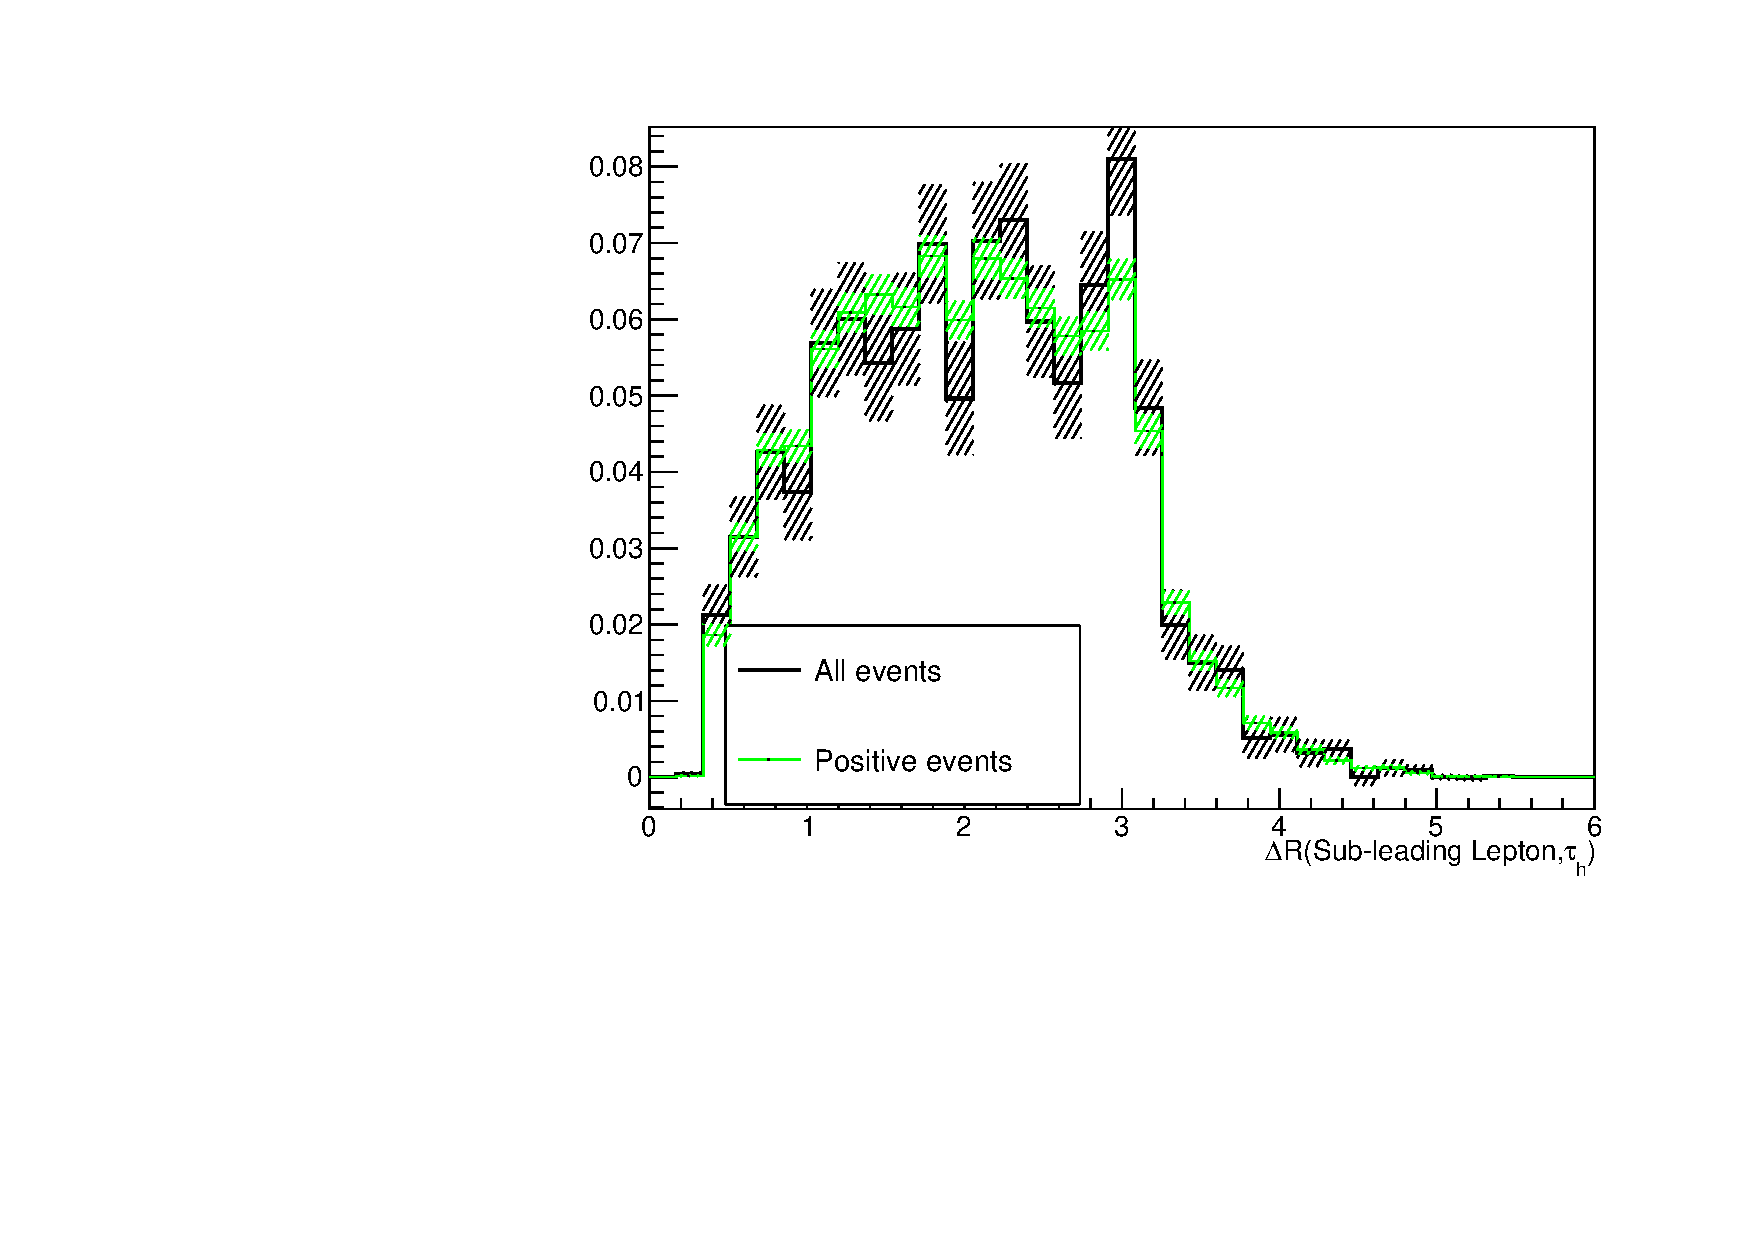
\includegraphics[width=.99\linewidth]{Appendices/Appendix_NegativeWeigts/PosVsAll_SS_err_deltaR_tau_LightLep2}
  \caption{$\Delta R$(\tauhad, sub-leading light-favoured lepton)}
\end{subfigure}%
\caption{Some normalised distributions for all the signal events in the \dilepSStau (black) and just the positively weighted events (green).  For each bin, the error band is calculated as the square root of the quadratic sum of the weights.}
\label{fig:Appendix:NegWeights:Distributions}
\end{figure}
% Plots produced with /lhome/ific/p/pamarag/Work/data/Draw3r.py
% https://ned.ipac.caltech.edu/level5/Leo/Stats_contents.html


\subsection{Errors in binned histograms}
If a bin of a histogram has $n$ entries of weighted events $w_i$ with $i=1, 2, ..., n$, the 
size of the bar is $\sum_{i=1}^{n} w_i$. Therefore, the error of that bar is 
\begin{equation}
\sqrt{\sum_{i=1}^{n} w^{2}_{i}}
\end{equation}

This expression for the error of a bin in a histogram is based on error propagation and intrinsic poissonian statistics only.
The variance, i.e.  the error on the weighted number of events" in that bin, is given by error propagation:
\begin{equation*}
V(\sum_{i=1}^{n} w_i) = \sqrt{(\sum_{i=1}^{n} w^{2}_{i}})^{2} = \sum_{i=1}^{n} w^{2}_{i} = \sum_{i=1}^{n}  V(w_i)
\end{equation*}
The variance of the weight $w_i$, $V(w_i)$, is determined only by the statistical fluctuation of the number of events 
considered: $V(w_{i}) =w^{2}_{i}$. 
% Why the bin error for weighted histogram is equal to the square root of their the sum of the 
% bin weight square https://www-zeuthen.desy.de/~wischnew/amanda/discussion/wgterror/working.html


\section{Negative weights in MVA methods}
Events coming from the MC generator can be produced with (unphysical) negative weights in some phase-space 
regions. Such occurrences are frequently inconvenient to deal with, and whether or not they are handled effectively 
is dependent on the MVA method's actual implementation. 
Within the ROOT TMVA library, probability and multi-dimensional probability density 
estimators, as well as BDTs, are among the methods that correctly include occurrences with negative weights.
In cases where a method does not properly treat events with negative weights, it is advisable to ignore such events 
for the training but to include them in the performance evaluation to not bias the results.

%POSTAMBLE
\begin{comment}
asdf
%\end{document}
%ENDPOSTAMBLE
\end{comment}
